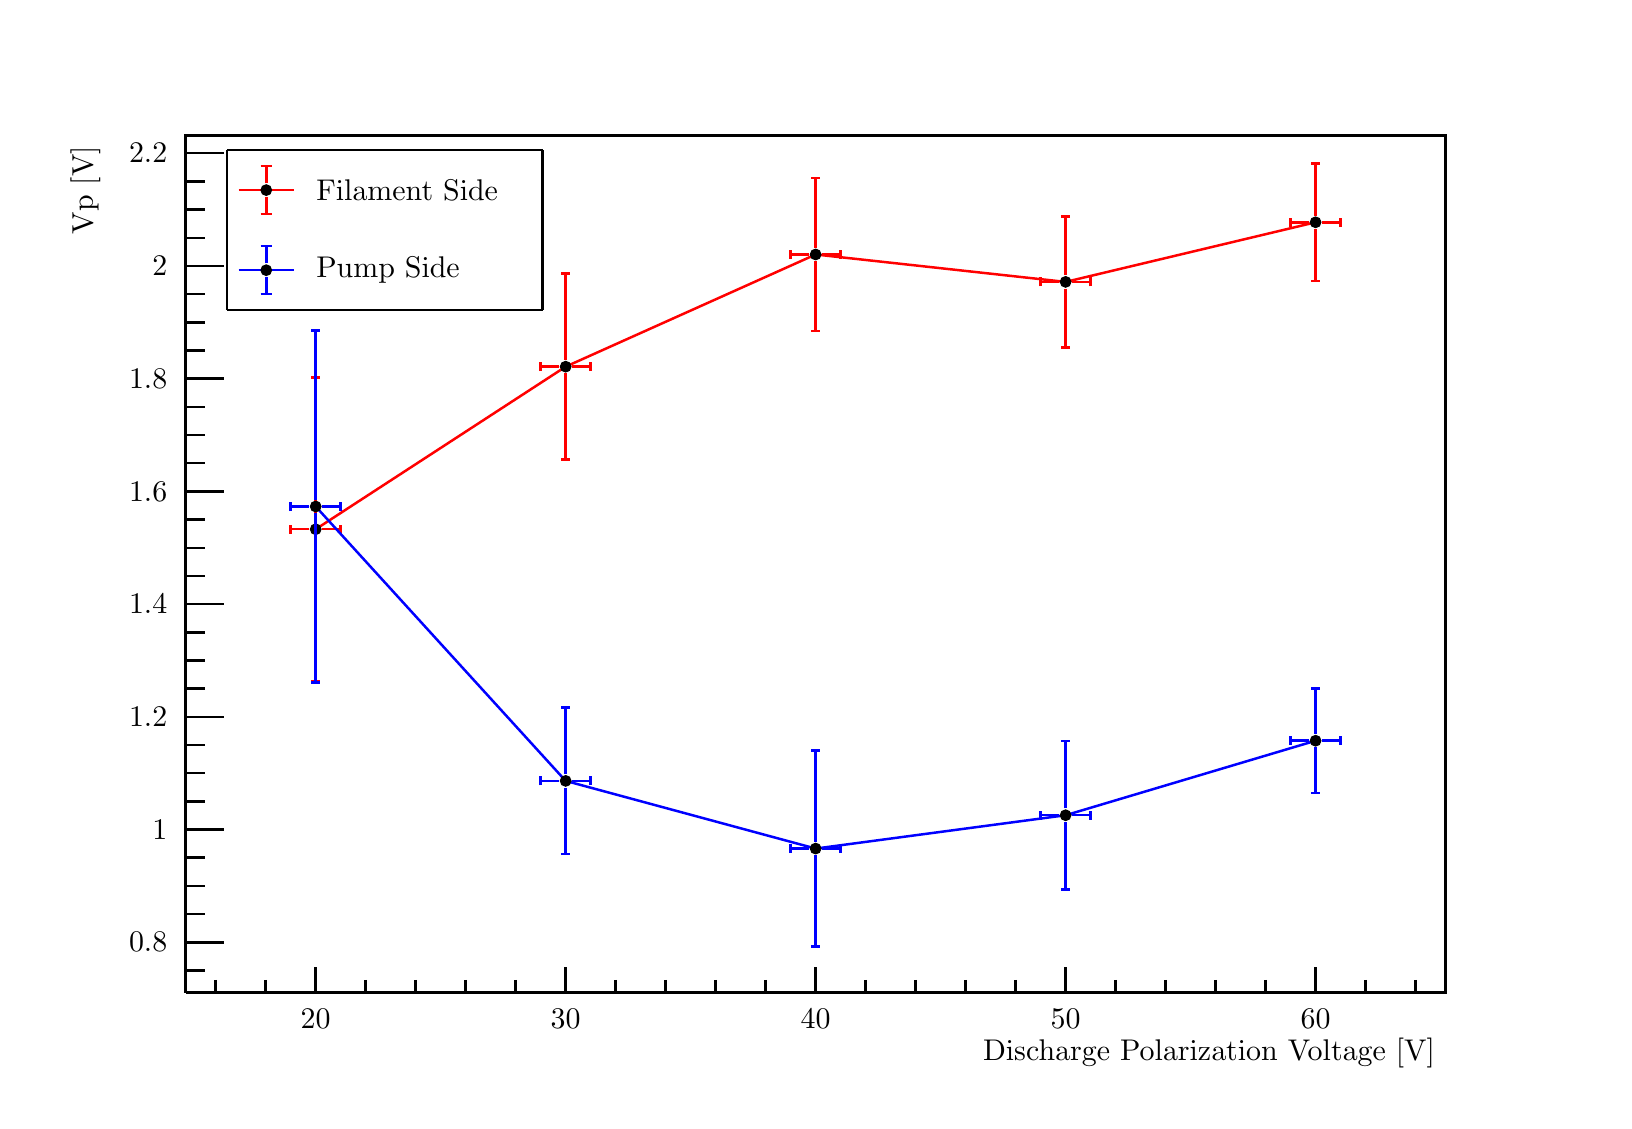
\begin{tikzpicture}
\pgfdeclareplotmark{cross} {
\pgfpathmoveto{\pgfpoint{-0.3\pgfplotmarksize}{\pgfplotmarksize}}
\pgfpathlineto{\pgfpoint{+0.3\pgfplotmarksize}{\pgfplotmarksize}}
\pgfpathlineto{\pgfpoint{+0.3\pgfplotmarksize}{0.3\pgfplotmarksize}}
\pgfpathlineto{\pgfpoint{+1\pgfplotmarksize}{0.3\pgfplotmarksize}}
\pgfpathlineto{\pgfpoint{+1\pgfplotmarksize}{-0.3\pgfplotmarksize}}
\pgfpathlineto{\pgfpoint{+0.3\pgfplotmarksize}{-0.3\pgfplotmarksize}}
\pgfpathlineto{\pgfpoint{+0.3\pgfplotmarksize}{-1.\pgfplotmarksize}}
\pgfpathlineto{\pgfpoint{-0.3\pgfplotmarksize}{-1.\pgfplotmarksize}}
\pgfpathlineto{\pgfpoint{-0.3\pgfplotmarksize}{-0.3\pgfplotmarksize}}
\pgfpathlineto{\pgfpoint{-1.\pgfplotmarksize}{-0.3\pgfplotmarksize}}
\pgfpathlineto{\pgfpoint{-1.\pgfplotmarksize}{0.3\pgfplotmarksize}}
\pgfpathlineto{\pgfpoint{-0.3\pgfplotmarksize}{0.3\pgfplotmarksize}}
\pgfpathclose
\pgfusepathqstroke
}
\pgfdeclareplotmark{cross*} {
\pgfpathmoveto{\pgfpoint{-0.3\pgfplotmarksize}{\pgfplotmarksize}}
\pgfpathlineto{\pgfpoint{+0.3\pgfplotmarksize}{\pgfplotmarksize}}
\pgfpathlineto{\pgfpoint{+0.3\pgfplotmarksize}{0.3\pgfplotmarksize}}
\pgfpathlineto{\pgfpoint{+1\pgfplotmarksize}{0.3\pgfplotmarksize}}
\pgfpathlineto{\pgfpoint{+1\pgfplotmarksize}{-0.3\pgfplotmarksize}}
\pgfpathlineto{\pgfpoint{+0.3\pgfplotmarksize}{-0.3\pgfplotmarksize}}
\pgfpathlineto{\pgfpoint{+0.3\pgfplotmarksize}{-1.\pgfplotmarksize}}
\pgfpathlineto{\pgfpoint{-0.3\pgfplotmarksize}{-1.\pgfplotmarksize}}
\pgfpathlineto{\pgfpoint{-0.3\pgfplotmarksize}{-0.3\pgfplotmarksize}}
\pgfpathlineto{\pgfpoint{-1.\pgfplotmarksize}{-0.3\pgfplotmarksize}}
\pgfpathlineto{\pgfpoint{-1.\pgfplotmarksize}{0.3\pgfplotmarksize}}
\pgfpathlineto{\pgfpoint{-0.3\pgfplotmarksize}{0.3\pgfplotmarksize}}
\pgfpathclose
\pgfusepathqfillstroke
}
\pgfdeclareplotmark{newstar} {
\pgfpathmoveto{\pgfqpoint{0pt}{\pgfplotmarksize}}
\pgfpathlineto{\pgfqpointpolar{44}{0.5\pgfplotmarksize}}
\pgfpathlineto{\pgfqpointpolar{18}{\pgfplotmarksize}}
\pgfpathlineto{\pgfqpointpolar{-20}{0.5\pgfplotmarksize}}
\pgfpathlineto{\pgfqpointpolar{-54}{\pgfplotmarksize}}
\pgfpathlineto{\pgfqpointpolar{-90}{0.5\pgfplotmarksize}}
\pgfpathlineto{\pgfqpointpolar{234}{\pgfplotmarksize}}
\pgfpathlineto{\pgfqpointpolar{198}{0.5\pgfplotmarksize}}
\pgfpathlineto{\pgfqpointpolar{162}{\pgfplotmarksize}}
\pgfpathlineto{\pgfqpointpolar{134}{0.5\pgfplotmarksize}}
\pgfpathclose
\pgfusepathqstroke
}
\pgfdeclareplotmark{newstar*} {
\pgfpathmoveto{\pgfqpoint{0pt}{\pgfplotmarksize}}
\pgfpathlineto{\pgfqpointpolar{44}{0.5\pgfplotmarksize}}
\pgfpathlineto{\pgfqpointpolar{18}{\pgfplotmarksize}}
\pgfpathlineto{\pgfqpointpolar{-20}{0.5\pgfplotmarksize}}
\pgfpathlineto{\pgfqpointpolar{-54}{\pgfplotmarksize}}
\pgfpathlineto{\pgfqpointpolar{-90}{0.5\pgfplotmarksize}}
\pgfpathlineto{\pgfqpointpolar{234}{\pgfplotmarksize}}
\pgfpathlineto{\pgfqpointpolar{198}{0.5\pgfplotmarksize}}
\pgfpathlineto{\pgfqpointpolar{162}{\pgfplotmarksize}}
\pgfpathlineto{\pgfqpointpolar{134}{0.5\pgfplotmarksize}}
\pgfpathclose
\pgfusepathqfillstroke
}
\definecolor{c}{rgb}{1,1,1};
\draw [color=c, fill=c] (0,0) rectangle (20,13.6103);
\draw [color=c, fill=c] (2,1.36103) rectangle (18,12.2493);
\definecolor{c}{rgb}{0,0,0};
\draw [c,line width=0.9] (2,1.36103) -- (2,12.2493) -- (18,12.2493) -- (18,1.36103) -- (2,1.36103);
\definecolor{c}{rgb}{1,1,1};
\draw [color=c, fill=c] (2,1.36103) rectangle (18,12.2493);
\definecolor{c}{rgb}{0,0,0};
\draw [c,line width=0.9] (2,1.36103) -- (2,12.2493) -- (18,12.2493) -- (18,1.36103) -- (2,1.36103);
\draw [c,line width=0.9] (2,1.36103) -- (18,1.36103);
\draw [c,line width=0.9] (3.65079,1.68768) -- (3.65079,1.36103);
\draw [c,line width=0.9] (4.28571,1.52436) -- (4.28571,1.36103);
\draw [c,line width=0.9] (4.92064,1.52436) -- (4.92064,1.36103);
\draw [c,line width=0.9] (5.55556,1.52436) -- (5.55556,1.36103);
\draw [c,line width=0.9] (6.19048,1.52436) -- (6.19048,1.36103);
\draw [c,line width=0.9] (6.8254,1.68768) -- (6.8254,1.36103);
\draw [c,line width=0.9] (7.46032,1.52436) -- (7.46032,1.36103);
\draw [c,line width=0.9] (8.09524,1.52436) -- (8.09524,1.36103);
\draw [c,line width=0.9] (8.73016,1.52436) -- (8.73016,1.36103);
\draw [c,line width=0.9] (9.36508,1.52436) -- (9.36508,1.36103);
\draw [c,line width=0.9] (10,1.68768) -- (10,1.36103);
\draw [c,line width=0.9] (10.6349,1.52436) -- (10.6349,1.36103);
\draw [c,line width=0.9] (11.2698,1.52436) -- (11.2698,1.36103);
\draw [c,line width=0.9] (11.9048,1.52436) -- (11.9048,1.36103);
\draw [c,line width=0.9] (12.5397,1.52436) -- (12.5397,1.36103);
\draw [c,line width=0.9] (13.1746,1.68768) -- (13.1746,1.36103);
\draw [c,line width=0.9] (13.8095,1.52436) -- (13.8095,1.36103);
\draw [c,line width=0.9] (14.4444,1.52436) -- (14.4444,1.36103);
\draw [c,line width=0.9] (15.0794,1.52436) -- (15.0794,1.36103);
\draw [c,line width=0.9] (15.7143,1.52436) -- (15.7143,1.36103);
\draw [c,line width=0.9] (16.3492,1.68768) -- (16.3492,1.36103);
\draw [c,line width=0.9] (3.65079,1.68768) -- (3.65079,1.36103);
\draw [c,line width=0.9] (3.01587,1.52436) -- (3.01587,1.36103);
\draw [c,line width=0.9] (2.38095,1.52436) -- (2.38095,1.36103);
\draw [c,line width=0.9] (16.3492,1.68768) -- (16.3492,1.36103);
\draw [c,line width=0.9] (16.9841,1.52436) -- (16.9841,1.36103);
\draw [c,line width=0.9] (17.619,1.52436) -- (17.619,1.36103);
\draw [anchor=base] (3.65079,0.911891) node[scale=1.08185, color=c, rotate=0]{20};
\draw [anchor=base] (6.8254,0.911891) node[scale=1.08185, color=c, rotate=0]{30};
\draw [anchor=base] (10,0.911891) node[scale=1.08185, color=c, rotate=0]{40};
\draw [anchor=base] (13.1746,0.911891) node[scale=1.08185, color=c, rotate=0]{50};
\draw [anchor=base] (16.3492,0.911891) node[scale=1.08185, color=c, rotate=0]{60};
\draw [anchor= east] (18,0.598854) node[scale=1.08185, color=c, rotate=0]{Discharge Polarization Voltage [V]};
\draw [c,line width=0.9] (2,1.36103) -- (2,12.2493);
\draw [c,line width=0.9] (2.48,2.00174) -- (2,2.00174);
\draw [c,line width=0.9] (2.24,2.35963) -- (2,2.35963);
\draw [c,line width=0.9] (2.24,2.71753) -- (2,2.71753);
\draw [c,line width=0.9] (2.24,3.07543) -- (2,3.07543);
\draw [c,line width=0.9] (2.48,3.43333) -- (2,3.43333);
\draw [c,line width=0.9] (2.24,3.79122) -- (2,3.79122);
\draw [c,line width=0.9] (2.24,4.14912) -- (2,4.14912);
\draw [c,line width=0.9] (2.24,4.50702) -- (2,4.50702);
\draw [c,line width=0.9] (2.48,4.86492) -- (2,4.86492);
\draw [c,line width=0.9] (2.24,5.22282) -- (2,5.22282);
\draw [c,line width=0.9] (2.24,5.58071) -- (2,5.58071);
\draw [c,line width=0.9] (2.24,5.93861) -- (2,5.93861);
\draw [c,line width=0.9] (2.48,6.29651) -- (2,6.29651);
\draw [c,line width=0.9] (2.24,6.65441) -- (2,6.65441);
\draw [c,line width=0.9] (2.24,7.0123) -- (2,7.0123);
\draw [c,line width=0.9] (2.24,7.3702) -- (2,7.3702);
\draw [c,line width=0.9] (2.48,7.7281) -- (2,7.7281);
\draw [c,line width=0.9] (2.24,8.086) -- (2,8.086);
\draw [c,line width=0.9] (2.24,8.4439) -- (2,8.4439);
\draw [c,line width=0.9] (2.24,8.80179) -- (2,8.80179);
\draw [c,line width=0.9] (2.48,9.15969) -- (2,9.15969);
\draw [c,line width=0.9] (2.24,9.51759) -- (2,9.51759);
\draw [c,line width=0.9] (2.24,9.87549) -- (2,9.87549);
\draw [c,line width=0.9] (2.24,10.2334) -- (2,10.2334);
\draw [c,line width=0.9] (2.48,10.5913) -- (2,10.5913);
\draw [c,line width=0.9] (2.24,10.9492) -- (2,10.9492);
\draw [c,line width=0.9] (2.24,11.3071) -- (2,11.3071);
\draw [c,line width=0.9] (2.24,11.665) -- (2,11.665);
\draw [c,line width=0.9] (2.48,12.0229) -- (2,12.0229);
\draw [c,line width=0.9] (2.48,2.00174) -- (2,2.00174);
\draw [c,line width=0.9] (2.24,1.64384) -- (2,1.64384);
\draw [c,line width=0.9] (2.48,12.0229) -- (2,12.0229);
\draw [anchor= east] (1.9,2.00174) node[scale=1.08185, color=c, rotate=0]{0.8};
\draw [anchor= east] (1.9,3.43333) node[scale=1.08185, color=c, rotate=0]{1};
\draw [anchor= east] (1.9,4.86492) node[scale=1.08185, color=c, rotate=0]{1.2};
\draw [anchor= east] (1.9,6.29651) node[scale=1.08185, color=c, rotate=0]{1.4};
\draw [anchor= east] (1.9,7.7281) node[scale=1.08185, color=c, rotate=0]{1.6};
\draw [anchor= east] (1.9,9.15969) node[scale=1.08185, color=c, rotate=0]{1.8};
\draw [anchor= east] (1.9,10.5913) node[scale=1.08185, color=c, rotate=0]{2};
\draw [anchor= east] (1.9,12.0229) node[scale=1.08185, color=c, rotate=0]{2.2};
\draw [anchor= east] (0.726934,12.2493) node[scale=1.08185, color=c, rotate=90]{Vp [V]};
\definecolor{c}{rgb}{1,0,0};
\draw [c,line width=0.9] (3.65079,7.24723) -- (6.8254,9.31201) -- (10,10.7367) -- (13.1746,10.3885) -- (16.3492,11.1456);
\definecolor{c}{rgb}{0,0,0};
\foreach \P in {(3.65079,7.24723), (6.8254,9.31201), (10,10.7367), (13.1746,10.3885), (16.3492,11.1456)}{\draw[mark options={color=c,fill=c},mark size=1.921922pt,mark=*] plot coordinates {\P};}
\definecolor{c}{rgb}{1,0,0};
\draw [c,line width=0.9] (3.56483,7.24723) -- (3.33333,7.24723);
\draw [c,line width=0.9] (3.33333,7.18992) -- (3.33333,7.30453);
\draw [c,line width=0.9] (3.73675,7.24723) -- (3.96825,7.24723);
\draw [c,line width=0.9] (3.96825,7.18992) -- (3.96825,7.30453);
\draw [c,line width=0.9] (3.65079,7.33319) -- (3.65079,9.17309);
\draw [c,line width=0.9] (3.59349,9.17309) -- (3.7081,9.17309);
\draw [c,line width=0.9] (3.65079,7.16127) -- (3.65079,5.32137);
\draw [c,line width=0.9] (3.59349,5.32137) -- (3.7081,5.32137);
\draw [c,line width=0.9] (6.73944,9.31201) -- (6.50794,9.31201);
\draw [c,line width=0.9] (6.50794,9.25471) -- (6.50794,9.36932);
\draw [c,line width=0.9] (6.91136,9.31201) -- (7.14286,9.31201);
\draw [c,line width=0.9] (7.14286,9.25471) -- (7.14286,9.36932);
\draw [c,line width=0.9] (6.8254,9.39797) -- (6.8254,10.4926);
\draw [c,line width=0.9] (6.76809,10.4926) -- (6.8827,10.4926);
\draw [c,line width=0.9] (6.8254,9.22605) -- (6.8254,8.13142);
\draw [c,line width=0.9] (6.76809,8.13142) -- (6.8827,8.13142);
\draw [c,line width=0.9] (9.91404,10.7367) -- (9.68254,10.7367);
\draw [c,line width=0.9] (9.68254,10.6794) -- (9.68254,10.794);
\draw [c,line width=0.9] (10.086,10.7367) -- (10.3175,10.7367);
\draw [c,line width=0.9] (10.3175,10.6794) -- (10.3175,10.794);
\draw [c,line width=0.9] (10,10.8226) -- (10,11.7111);
\draw [c,line width=0.9] (9.94269,11.7111) -- (10.0573,11.7111);
\draw [c,line width=0.9] (10,10.6507) -- (10,9.76223);
\draw [c,line width=0.9] (9.94269,9.76223) -- (10.0573,9.76223);
\draw [c,line width=0.9] (13.0886,10.3885) -- (12.8571,10.3885);
\draw [c,line width=0.9] (12.8571,10.3312) -- (12.8571,10.4458);
\draw [c,line width=0.9] (13.2606,10.3885) -- (13.4921,10.3885);
\draw [c,line width=0.9] (13.4921,10.3312) -- (13.4921,10.4458);
\draw [c,line width=0.9] (13.1746,10.4745) -- (13.1746,11.2211);
\draw [c,line width=0.9] (13.1173,11.2211) -- (13.2319,11.2211);
\draw [c,line width=0.9] (13.1746,10.3025) -- (13.1746,9.55585);
\draw [c,line width=0.9] (13.1173,9.55585) -- (13.2319,9.55585);
\draw [c,line width=0.9] (16.2632,11.1456) -- (16.0317,11.1456);
\draw [c,line width=0.9] (16.0317,11.0883) -- (16.0317,11.2029);
\draw [c,line width=0.9] (16.4352,11.1456) -- (16.6667,11.1456);
\draw [c,line width=0.9] (16.6667,11.0883) -- (16.6667,11.2029);
\draw [c,line width=0.9] (16.3492,11.2316) -- (16.3492,11.8907);
\draw [c,line width=0.9] (16.2919,11.8907) -- (16.4065,11.8907);
\draw [c,line width=0.9] (16.3492,11.0596) -- (16.3492,10.4005);
\draw [c,line width=0.9] (16.2919,10.4005) -- (16.4065,10.4005);
\definecolor{c}{rgb}{0,0,1};
\draw [c,line width=0.9] (3.56483,7.5362) -- (3.33333,7.5362);
\draw [c,line width=0.9] (3.33333,7.47889) -- (3.33333,7.5935);
\draw [c,line width=0.9] (3.73675,7.5362) -- (3.96825,7.5362);
\draw [c,line width=0.9] (3.96825,7.47889) -- (3.96825,7.5935);
\draw [c,line width=0.9] (3.65079,7.62216) -- (3.65079,9.77439);
\draw [c,line width=0.9] (3.59349,9.77439) -- (3.7081,9.77439);
\draw [c,line width=0.9] (3.65079,7.45024) -- (3.65079,5.298);
\draw [c,line width=0.9] (3.59349,5.298) -- (3.7081,5.298);
\draw [c,line width=0.9] (6.73944,4.05127) -- (6.50794,4.05127);
\draw [c,line width=0.9] (6.50794,3.99397) -- (6.50794,4.10858);
\draw [c,line width=0.9] (6.91136,4.05127) -- (7.14286,4.05127);
\draw [c,line width=0.9] (7.14286,3.99397) -- (7.14286,4.10858);
\draw [c,line width=0.9] (6.8254,4.13723) -- (6.8254,4.98096);
\draw [c,line width=0.9] (6.76809,4.98096) -- (6.8827,4.98096);
\draw [c,line width=0.9] (6.8254,3.96531) -- (6.8254,3.12158);
\draw [c,line width=0.9] (6.76809,3.12158) -- (6.8827,3.12158);
\draw [c,line width=0.9] (9.91404,3.19187) -- (9.68254,3.19187);
\draw [c,line width=0.9] (9.68254,3.13457) -- (9.68254,3.24918);
\draw [c,line width=0.9] (10.086,3.19187) -- (10.3175,3.19187);
\draw [c,line width=0.9] (10.3175,3.13457) -- (10.3175,3.24918);
\draw [c,line width=0.9] (10,3.27783) -- (10,4.4355);
\draw [c,line width=0.9] (9.94269,4.4355) -- (10.0573,4.4355);
\draw [c,line width=0.9] (10,3.10591) -- (10,1.94824);
\draw [c,line width=0.9] (9.94269,1.94824) -- (10.0573,1.94824);
\draw [c,line width=0.9] (13.0886,3.61528) -- (12.8571,3.61528);
\draw [c,line width=0.9] (12.8571,3.55798) -- (12.8571,3.67259);
\draw [c,line width=0.9] (13.2606,3.61528) -- (13.4921,3.61528);
\draw [c,line width=0.9] (13.4921,3.55798) -- (13.4921,3.67259);
\draw [c,line width=0.9] (13.1746,3.70124) -- (13.1746,4.55578);
\draw [c,line width=0.9] (13.1173,4.55578) -- (13.2319,4.55578);
\draw [c,line width=0.9] (13.1746,3.52932) -- (13.1746,2.67478);
\draw [c,line width=0.9] (13.1173,2.67478) -- (13.2319,2.67478);
\draw [c,line width=0.9] (16.2632,4.56156) -- (16.0317,4.56156);
\draw [c,line width=0.9] (16.0317,4.50426) -- (16.0317,4.61887);
\draw [c,line width=0.9] (16.4352,4.56156) -- (16.6667,4.56156);
\draw [c,line width=0.9] (16.6667,4.50426) -- (16.6667,4.61887);
\draw [c,line width=0.9] (16.3492,4.64752) -- (16.3492,5.2277);
\draw [c,line width=0.9] (16.2919,5.2277) -- (16.4065,5.2277);
\draw [c,line width=0.9] (16.3492,4.4756) -- (16.3492,3.89542);
\draw [c,line width=0.9] (16.2919,3.89542) -- (16.4065,3.89542);
\draw [c,line width=0.9] (3.65079,7.5362) -- (6.8254,4.05127) -- (10,3.19187) -- (13.1746,3.61528) -- (16.3492,4.56156);
\definecolor{c}{rgb}{0,0,0};
\foreach \P in {(3.65079,7.5362), (6.8254,4.05127), (10,3.19187), (13.1746,3.61528), (16.3492,4.56156)}{\draw[mark options={color=c,fill=c},mark size=1.921922pt,mark=*] plot coordinates {\P};}
\definecolor{c}{rgb}{1,1,1};
\draw [color=c, fill=c] (2.52149,10.0287) rectangle (6.53295,12.063);
\definecolor{c}{rgb}{0,0,0};
\draw [c,line width=0.9] (2.52149,10.0287) -- (6.53295,10.0287);
\draw [c,line width=0.9] (6.53295,10.0287) -- (6.53295,12.063);
\draw [c,line width=0.9] (6.53295,12.063) -- (2.52149,12.063);
\draw [c,line width=0.9] (2.52149,12.063) -- (2.52149,10.0287);
\draw [anchor= west] (3.52436,11.5544) node[scale=1.08185, color=c, rotate=0]{Filament Side};
\definecolor{c}{rgb}{1,0,0};
\draw [c,line width=0.9] (2.67192,11.5544) -- (3.37393,11.5544);
\draw [c,line width=0.9] (3.02292,11.6404) -- (3.02292,11.8596);
\draw [c,line width=0.9] (3.02292,11.4685) -- (3.02292,11.2493);
\draw [c,line width=0.9] (2.95272,11.8596) -- (3.09312,11.8596);
\draw [c,line width=0.9] (2.95272,11.2493) -- (3.09312,11.2493);
\definecolor{c}{rgb}{0,0,0};
\foreach \P in {(3.02292,11.5544)}{\draw[mark options={color=c,fill=c},mark size=1.921922pt,mark=*] plot coordinates {\P};}
\draw [anchor= west] (3.52436,10.5372) node[scale=1.08185, color=c, rotate=0]{Pump Side};
\definecolor{c}{rgb}{0,0,1};
\draw [c,line width=0.9] (2.67192,10.5372) -- (3.37393,10.5372);
\draw [c,line width=0.9] (3.02292,10.6232) -- (3.02292,10.8424);
\draw [c,line width=0.9] (3.02292,10.4513) -- (3.02292,10.2321);
\draw [c,line width=0.9] (2.95272,10.8424) -- (3.09312,10.8424);
\draw [c,line width=0.9] (2.95272,10.2321) -- (3.09312,10.2321);
\definecolor{c}{rgb}{0,0,0};
\foreach \P in {(3.02292,10.5372)}{\draw[mark options={color=c,fill=c},mark size=1.921922pt,mark=*] plot coordinates {\P};}
\end{tikzpicture}
